\documentclass[10pt]{extarticle} % article doctype, possible font size range from 8pt to 20pt with not all being avaiable.
\title{Game AAI Assignment}
\author{Tim Hintzbergen and Sjoerd Dekker}
\date{March 2018}
% include packages
\usepackage{graphicx}
\usepackage{caption}
\usepackage{mathabx}
\usepackage[margin=1.0in]{geometry} % Sets page margin, 2.0in is default.
\DeclareCaptionFormat{cancaption}{#1#2#3\par} % Normal format actually
\DeclareCaptionLabelFormat{cancaptionlabel}{#1}
\captionsetup[figure][number]{format=cancaption,labelformat=cancaptionlabel}
\graphicspath { {images/} }
\begin{document}
   \maketitle
   \thispagestyle{empty}
   \newpage
      %------------------------------------------------------------------------------------------------------------------------------------------------------- Introduction
   \newpage
   \setcounter{page}{1}
   \section {Introduction}
   This paper contains the documentation of the final assignment of the course Algorithms and Artificial Intelligence for Games. The task of this assignment was to build a game or simulation containing certain aspected that were taught during the course, namely:
   \begin{itemize}
      \item Steering behaviours
      \item Pathfinding
      \item States and scripting
      \item Fuzzy logic
   \end{itemize}
   The premises of the application was a simulation of different animals and evolution. But soon due to time constraints the project turned out more as a toolbox styled with the natural world. The original idea was to contain evolving herbivores that had a certain fitness. Carnivores would then hunt the herbivores. Depending on the fitness certain herbivores could survive, and produce offspring, thereby passing on part of their fitness to their young.
   \newpage

   \tableofcontents{}
   \newpage
   %------------------------------------------------------------------------------------------------------------------------------------------------------- Steering behaviours
   \section{Steering behaviours}
   The following steering behaviours are implemented. 
   \subsection{Simple steering behaviours}
   \subsubsection {Arrive}
   The entity will try to go in a straight line to a specified goal. When the entity gets close to the goal the entity will slow down. This behaviour will stop when the entity is on or very near its goal and the current speed of the entity is very low. 
   \subsubsection {Flee}
   The entity will try to run away from entities that are the of the type specified. The closer another entity is the more the current entity will try to run away from the other entity. This algorithm will only search in a certain area, if there are no entities in the area the entity will not try to run away.
   \subsubsection {Seek}
   This algorithm has the opposite behaviour from flee. However in this algorithm there is only one entity set to seek. If the specified entity to seek is to far away, then this behaviour will terminate itself.
   \subsubsection {Wander}
  This algorithm will create a circle in front of the entity, on this circle there is a dot. This dot will move randomly along the circle. The entity will go towards the dot, the farther away the dot is from the entity the more force is applied. 
  \subsection{Advanced steering behaviours}
  \subsubsection {Flocking}
  First all entities of the same type are searched in a radius around the current entity, exluding itself. The current entity will do the following three behaviours: 
  \begin{itemize}
  \item Alignment: the entity will calculate the average direction off all the entities in the area. After this the entity will try to have the same direction as the average.
  \item Cohesion: the entity will try gravitate towards the average location of all the entities in the area.
  \item Separation: the entity  will try to go away from all the entities in the area. 
  \end{itemize}
  \subsubsection {Obstacle avoidance}
  First all obstacles are searched within a radius (default 60 units) around the entity. For every object the angle from the entity to the object and the direction of the entity are compared. If the difference is more than 90$^{\circ}$ then the object is ignored. For the remaining obstacles the distance at the closest point (if the entity keeps moving in a straight line) between the entity and the obstacle is calculated. If this distance is less then \(radius of obstacle + radius of entity\), then this behaviour will add a force to the entity to try to avoid the obstacle.
  \subsubsection {Path following}
   This algorithm will create a path to a specified location using the A* algorithm. But only if the goal is not in plain view. After the A* algorithm has found a path then this path will be smoothed. When the smoothing is done the agent will follow the path. This is done using the arrive algorithm. 
   \newpage
   
   %------------------------------------------------------------------------------------------------------------------------------------------------------- Pathfinding
   \section {Pathfinding}
This section will explain all techniques used in regard to pathfinding.
   \subsection {Graph}
  A graph is used as underlying structure to allow pathfinding. Graph is a singleton and is its vertices are build along a grid of with a fixed cardinal distance between each vertex. Every time a vertex is placed the instantiation algorithm will determine if an agent will fit on that vertex without colliding with nearby obstancles. This is once again performed when all vertices are chained together with edges. The algorithm checks if the new edge is walkable for an entity before stitching vertices together using that edge.\\
   Various settings like spacing between vertices can be set in the settings.ini file. Furthermore graph can be rendered to the screen by clicking the \emph{navigation} option under the \emph{view} button.
   \subsection {A*}
  Our application only uses A* since pathfinding is only used to travel to single locations. In fact there are two different A* implementation, the first one will be explained here, the second one will be discussed in the section \ref{tsastar}.\\
  A* uses a heuristic based on the type of graph created. If there are only cardinal edges then the manhattan distance will be used. Otherwise the heuristic will use the euclidian distance. A* will prioritize its search through the use of a priority queue based on an array that sorts every new entry based on the heuristic cost. 
   \subsection {Path smoothing}
A modified approach to the precise path smoothing algorithm of Mat Buckland \cite{pgaie} is used. This modified approach was suggested by a fellow student during the course. In our case there are few obstacles that an pathplanning agent needs to avoid, and therefore path smoothing from the first vertex to the goal vertex is always an \(O(n)\) best-case operation. To make path smoothing slightly more efficient path smoothing is performed backwards, evaluating from the goal vertex back to the agent its location. This results in the same worst-case operation, but a better average and best-case operation.\\
   Path smoothing can be disabled in the settings.ini files.
   \subsection {Time slicing} \label{tsastar}
  When multiple agents need to calculate a path in the game world the whole application would lock until they all received their path. To avoid this a new pathfollowing behaviour is created to communicate with a global pathplanning manager. The manager manages all pathfinding requests and distributes its resources equally among all requests. A observer pattern is used to register and unregister seperate path planners to the path planning manager.
   The path planning manager can be rendered to the screen by clicking the \emph{Path Planning Manager} option under the \emph{view} button.
   \newpage   
   %------------------------------------------------------------------------------------------------------------------------------------------------------- States
   \section {States}
   The simulation uses states to determine what the entities should be doing. Each entity keeps track of its own state and the previous state. In figure~\ref{fig:stateClassDiagram} the relevant classes' properties and methods are shown.
   \begin{figure}[h!]
   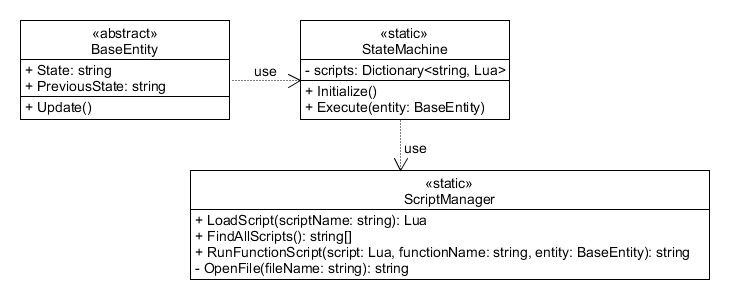
\includegraphics[width=\textwidth]{stateuml.png}
   \caption{State class diagram}
   \label{fig:stateClassDiagram}
   \end{figure}
   \\When the simulation is started the Initialize method in StateMachine is called, this will preload all the scripts. All scripts are located in the scripts folder. The scripts are seperated into folders, each folder is linked, based on the name, to an entity type.
   The default states for every entity type are set in the settings.ini file.
   \subsection {Scripting}
   States are scripted in Lua. Each state for every entity type has its own script file. Each file has to have at least three functions: 
   \begin{itemize}
   \item enter(entity, world). This function is called when the entity switches to this state. In this function the necessary steeringbehaviours are added to the entity.
   \item execute(entity, world). This function is called on every tick that the state is active. This function should update relevant values for the entity. This function has to return the new state as a string, if the state should not change then it has to return the name of the current state.
   \item exit(entity, world). This function is called when the entity leaves this state. In here, if necessary, the steering behaviours should be removed.
   \end{itemize}
   The first parameter is the current entity, the second parameter is the gameworld instance. C\# namespaces can be imported in the scripts. This can be done by adding an import statement to the top of the script file, eg: \emph{import('System')}.
   
   When the simulation is running the BaseEntity Update method will call the StateMachine Execute method. The stateMachine execute method will call the necessary methods in the scripts using the RunFunctionScript method. If the state changes the exit function of the previous state and the enter function of the new state are executed.
   
   \newpage
   %------------------------------------------------------------------------------------------------------------------------------------------------------- Partitioning
   \section {Partitioning}
   The world is split into multiple cells. These cells are layed out in a grid pattern. The size of the cells can be set in the settings.ini file. An entity is always in one of these cells. When an entity moves the corrresponding cell in which the entity is located is recalculated. Searching for entities in an area works in the following manner (the area to search in is always a circle):
   \begin{enumerate}
   \item Calculate which cells, in a square, contain (some of) the area of the search circle.
   \item Get all the entities from the cells in step 1.
   \item for every entity calculate the distance from the center of the circle, if this is more than the radius of the circle then remove this entity.
   \end{enumerate}
   The cells can be rendered to the screen by clicking the \emph{spatialPartitioning Grid} option under the \emph{view} button. 
   
    \newpage
   %------------------------------------------------------------------------------------------------------------------------------------------------------- Fuzzy logic
   \section {Fuzzy logic}
   Fuzzy logic works in three steps. The values that go in and go out of the alghoritms are crisp values. All the graphs have a left and right shoulder and zero or more trapezoidal shaped sets. All the lines in the graph are either diagonal or horizontal.
   \subsection{Fuzzyfication}
   In this step the graphs are loaded from a text file (fuzzyrules/graphs.txt), this file is read on startup. For every graph these values need to be set: 
   \begin{itemize}
   \item MIN: the minimal value in the graph.
   \item MAX: the maximum value in the graph.
   \item SECTIONS: the names of the sets in the graph.
   \item SPACING: the values where the sets should stop and begin (there should be \( (section count) \times 2 - 2\) values in spacing). These values have to be in ascending order.
   \end{itemize}
   \subsection{Fuzzy rules}
   All rules are specified in a text file (fuzzyrules/rules.txt), this file is read on startup. For the ruleset the input graphs and output graph have to be specified. Only the \emph{and} statement is available in a rule, other statements like \emph{or} and \emph{not} are not available. An example ruleset is given in figure~\ref{fig:ruleset}.
   \begin{figure}[h!]
   {\ttfamily 
   		INPUTS = Ammo, Distance\\
  	 	OUTPUT = Weapon\\
   		IF Distance.Far AND Ammo.Loads THEN Weapon.Desirable \\
   		IF Distance.Far	AND Ammo.Okay THEN Weapon.Undesirable \\
   		IF Distance.Close AND Ammo.Okay THEN Weapon.Desirable \\
   		...
   }
   \caption{Example ruleset}
   \label{fig:ruleset}
   \end{figure}\\
   The execution for one rule works with these steps:
   \begin{enumerate}
   \item Get the value for every defined input set in the corresponding graph.
   \item Find the smallest value from step 1.
   \item Get the value for the defined set in the output graph.
   \item If the value from step 3 is smaller than the value from step 2 then update the value for the defined set in the output graph to the value from step 2.
   \end{enumerate}
   \subsection{Defuzzification}
   In the project there are three methods for defuzzification. The active method can be set in the settings.ini file.
   
   \subsubsection {Mean of maximum}  
   This method will calculate the average value for the set with the highest degree of membership. In figure~\ref{fig:MOM} the result would be \(\frac{73}{100}=86.5\). 
   \begin{figure}[h!]
   \begin{center}
   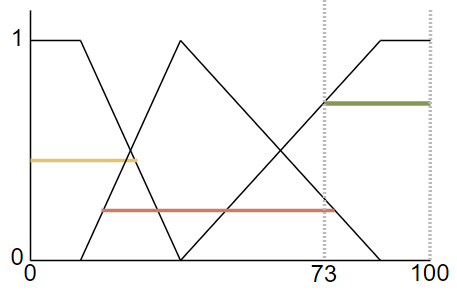
\includegraphics[width=7cm]{MOM.png}
   \end{center}
   \caption{Mean of maximum example}
   \label{fig:MOM}
   \end{figure}
   \subsubsection {Centroid}  
   This method will calculate the weighted average of the degree of membership (DOM) for an amount of locations. The amount of locations can be set in the settings.ini file.
   The result is calculated using the following formula:
   \[ result = \frac{\sum (DOM \times location)}{\sum DOM} \]
   
   \subsubsection {Average of maxima}  
   This method will calculate the average of the degree of membership for every set. An example is shown in figure~\ref{fig:maxAv}.
   \begin{figure}[h!]
   \begin{center}
   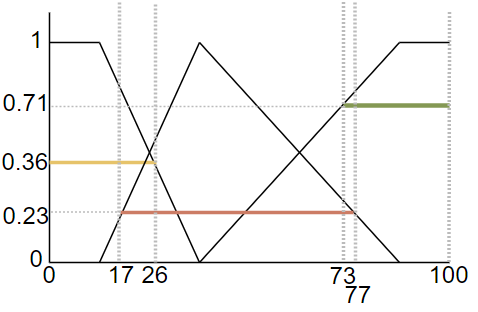
\includegraphics[width=7cm]{maxAv.png}
   \end{center}
   \[ result = \frac{0.36 \times ((0 + 26) / 2) + 0.23 \times ((17 + 77) / 2) + 0.71 \times ((73 + 100) / 2)}{0.36 + 0.23 + 0.71} = \frac{76.9}{1.3} = {59.16}\]
   \caption{Average of maxima example}
   \label{fig:maxAv}
   \end{figure}
   
\end{document}



\newpage
\bibliography{report} 
\bibliographystyle{ieeetr} % options: apalike for apa, ieeetr for ieee
\end{document}